\newpage
\section{Linear Regression}
\begin{flushleft}

Die lineare Regression ist ein Verfahren welches versucht, eine abhängige Variable durch eine oder mehrere unabhängige Variablen zu erklären.

\subsection{Simple lineare Regression}

Die simple lineare Regression arbeitet lediglich im zweidimensionalen Raum.

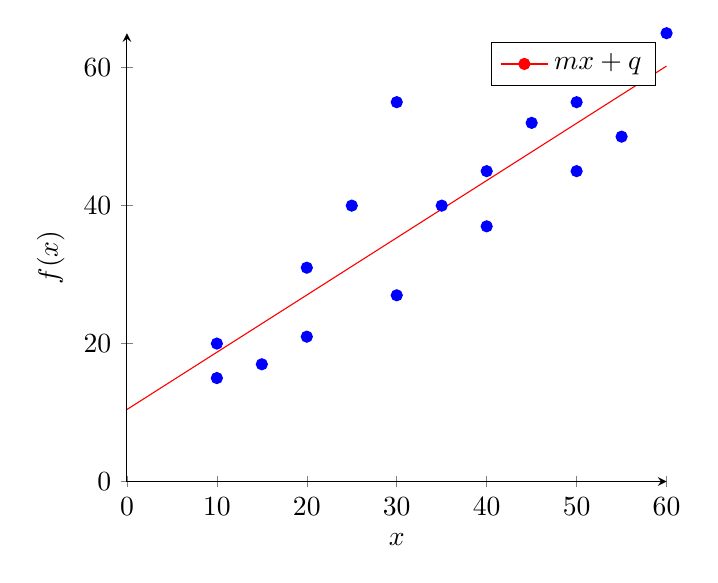
\begin{tikzpicture}
\begin{axis} [
	axis lines = left, % Only displays axis on left and bottom (not whole box)
	ymin = 0,	% y-axis shall always start at zero
	xlabel = $x$,
	ylabel = $f(x)$,
	mark=*,
	scatter/classes={%	Defines the point appearance for the scatter plot
		a={blue}%,
		%b={mark=triangle*,red},
		%c={mark=o,draw=black}
		}
	]

\addplot [
	domain = 0:60, 	% Range for the value x
	samples = 100,	% Determines the number of points in the interval defined by domain. 
	color = red,	% Color of the
	] {0.83*x + 10.44};
\addlegendentry {$mx + q$}

\addplot [only marks, scatter, scatter src=explicit symbolic]
	table [meta=class] {		% meta defines the column to use for the class of the point
		x		y		class
		10		20		a
		10		15		a
		15		17		a
		20		21		a
		20		31		a
		25		40		a
		30		27		a
		35		40		a
		30		55		a
		40		45		a
		40		37		a
		45		52		a
		50		55		a
		50		45		a
		55		50		a
		60		65		a
		
	};

\end{axis}
\end{tikzpicture}

Die Steigung [m] sowie der y-Achsenabschnitt [q] lassen sich wie folgt berechnen:

$$m = \dfrac{\sum_{i=1}^n (x_{i} - \bar{x})(y_{i} - \bar{y})}
                       {\sum_{i=1}^n (x_{i} - \bar{x})^{2}}$$

$$q = \bar{y} - m\bar{x}$$

Wobei die werte $\bar{x}$, $\bar{y}$ den arithmetischen Mitteln der Definitions- und Bildmenge entsprechen.
\linebreak
Die Qualität eines Regressionsmodells kann durch Genauigkeitsmetriken bestimmt werden. Hierbei werden stets die effektiven Y-Werte mit den jeweiligen Werten $\hat{y}_{i} = mx_{i} + q$ der linearen Regressionslinie verglichen.


Der \textbf{Mittlerer absoluter Fehler} (mean-absolute-error) ist die simpleste Metrik und zeig den effektiven Durchschnittsfehelr auf. 
$$MAE = \dfrac{1}{n}\sum_{i=1}^n|y_{i} - \hat{y}_{i}|$$


Die \textbf{Mittlere quadratische Abweichung} (mean-square-error) reagiert aufgrund des Exponenten proportional stärker auf grosse Fehler.
$$MSE = \dfrac{1}{n}\sum_{i=1}^n(y_{i} - \hat{y}_{i})^{2}$$

Der \textbf{root-mean-square-error} ist die gängigste Metrik, da dieser, durch das Ziehen der Wurzel, in der gleichen Einheit interpretierbar ist wie die eigentlichen Y-Vektoren.
$$RMSE = \sqrt{\dfrac{1}{n}\sum_{i=1}^n(y_{i} - \hat{y}_{i})^{2}} = \sqrt{MSE}$$


\subsection{Polynomial Regression}
\subsection{Multivariable Regression}

\end{flushleft}